\begin{savequote}[75mm]
Some Quote.
\qauthor{Quoteauthor Lastname}
\end{savequote}

%For an example of a full page figure, see Fig.~\ref{fig:myFullPageFigure}.
\chapter{Model-Based Point Cloud Tracking}
\label{Chap:ModelBasedTracking}
\lettrine[lines=3, loversize=0.3]{\textcolor{DarkBlue}N}{ow that we have established} a reduced, stable world model in which voxels persist through occlusions, the next step is to adapt the general framework of Sequential Bayesian Estimation to track models in this 3D voxel world. The core concepts remain the same as discussed in Chapter {Chap:VideoSegRelaxation}(for a brief introduction, see Appendix \ref{chap:SeqBayesEst}), and we will again use a bank of parallel particle filters, due to their robustness to noise (of which there is quite a bit in Kinect data) and ability to handle non-linear dynamics.

\section{Particle Filters in 3D}
\section{Model Representation}
\section{Measurement Model}
\section{Dynamic Model}
\section{KL-Divergence Adaptation}
\section{Stratified Correspondence Sampling}
\todo[inline]{Provide simple experiment showing quality of track (maybe on VR Data) vs number of samples and particles.}
\todo[inline]{Also show result with occlusion? With some pure random samples added in?}
\section{Results on Virtual-Reality Data}
\begin{figure*}[!ht]
  \centering
  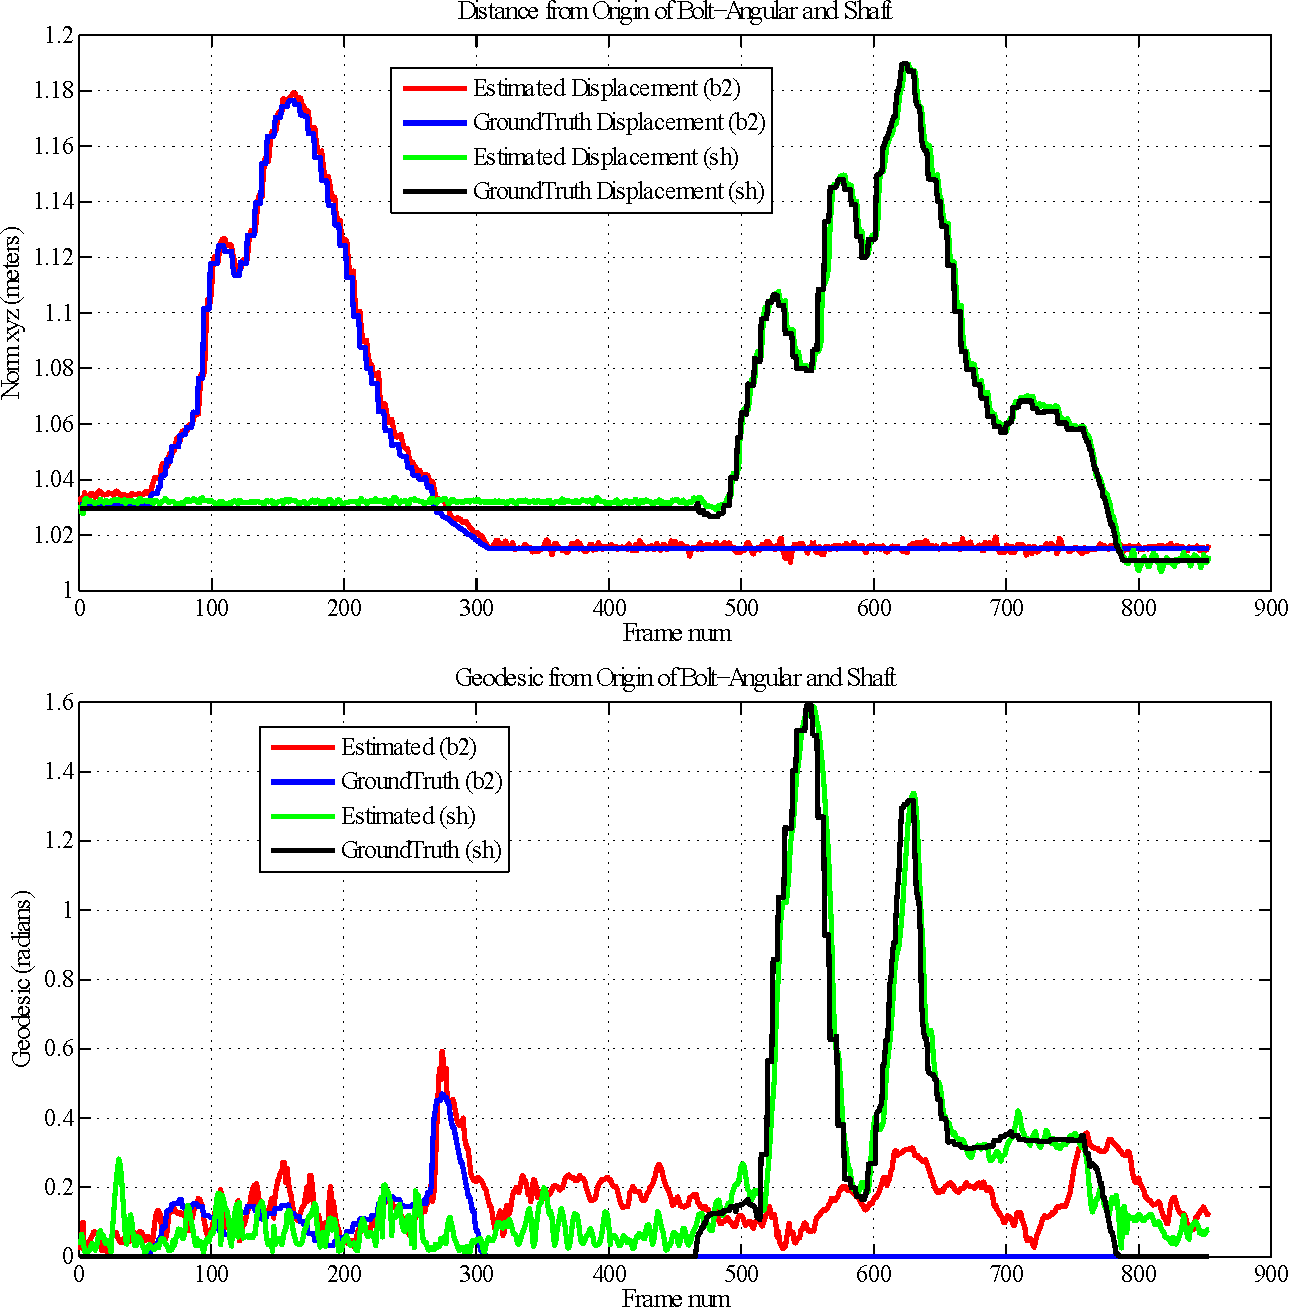
\includegraphics[width=\linewidth]{figures/Tracking/CombinedNoNoise.pdf}
  \caption[Tracked Output vs Ground Truth Artificial Sequence]{Tracked Output vs Ground Truth Artificial Sequence. The top panel shows position in terms of XYZ displacement and the bottom shows rotation in terms of geodesic. The location is generally tracked quite well, while the rotation is noisy due to the rotational symmetry of the two tracked objects (a bolt-angular and shaft).}
  \label{fig:CombinedNoNoise}
\end{figure*}

\begin{figure*}[!ht]
  \centering
  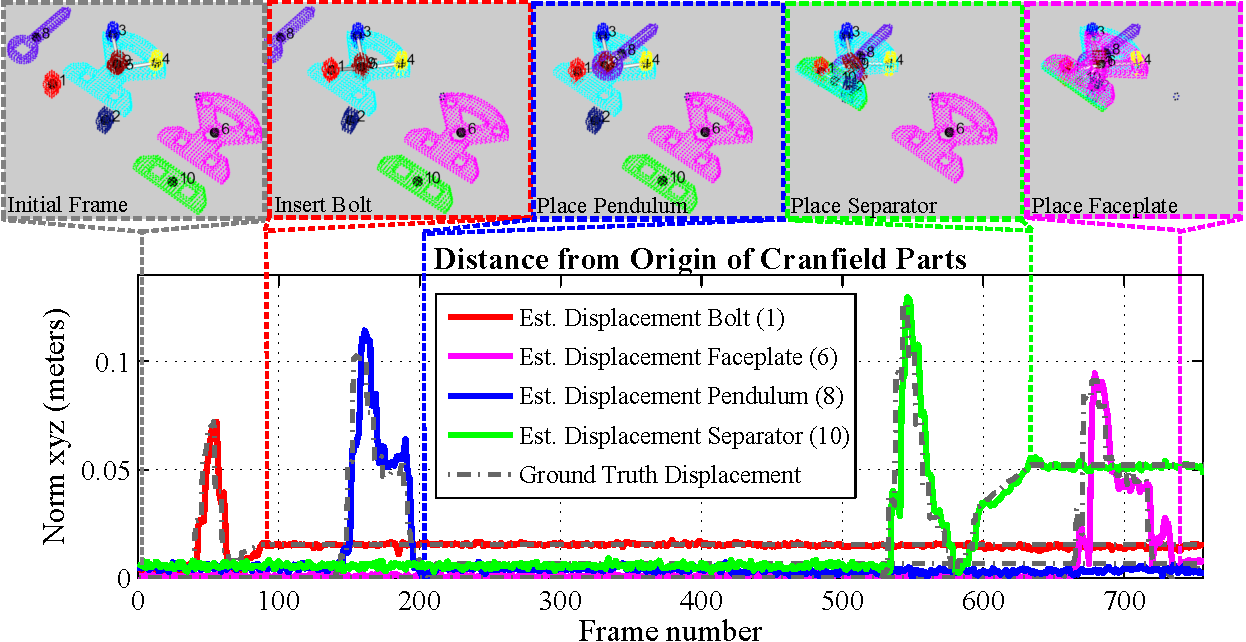
\includegraphics[width=\linewidth]{figures/Tracking/Action_Segmentation.pdf}
  \caption[Segmentation of Actions]{Segmentation of Cranfield Sequence into Keyframes - Tracked objects are monitored for when interactions between them occur, yielding keyframes which correspond to semantically important frames. Results here are shown for an artificial sequence with depth and RGB noise added.}
  \label{fig:ActionSegmentation}
\end{figure*}

\section{Results on Real Data}



